%%%%%%%%%%%%%%%%%%%%%%%%%%%%%%%%%%%%%%%%%
% Short Sectioned Assignment
% LaTeX Template
% Version 1.0 (5/5/12)
%
% This template has been downloaded from:
% http://www.LaTeXTemplates.com
%
% Original author:
% Frits Wenneker (http://www.howtotex.com)
%
% License:
% CC BY-NC-SA 3.0 (http://creativecommons.org/licenses/by-nc-sa/3.0/)
%
%%%%%%%%%%%%%%%%%%%%%%%%%%%%%%%%%%%%%%%%%

%----------------------------------------------------------------------------------------
%	PACKAGES AND OTHER DOCUMENT CONFIGURATIONS
%----------------------------------------------------------------------------------------

\documentclass[paper=a4, fontsize=11pt]{scrartcl} % A4 paper and 11pt font size

\usepackage[T1]{fontenc} % Use 8-bit encoding that has 256 glyphs
%\usepackage{fourier} % Use the Adobe Utopia font for the document - comment this line to return to the LaTeX default
\usepackage[english]{babel} % English language/hyphenation
\usepackage{amsmath,amsfonts,amsthm} % Math packages
\usepackage{mathtools} %More math! (For dscases)
\usepackage{hyperref} %HTML package
\usepackage{pgfplots} %Makes plots in LaTeX
\usepackage{tikz} %Also tikz?
\usepackage{bbm} %Blackboard bold 1
\usepgfplotslibrary{fillbetween}%Let's me fill between named plots
\usepackage{graphicx} %import pics
\graphicspath{ {Python_figs/} }
\DeclareGraphicsExtensions{.pdf,.png,.jpg}
\usepackage{sectsty} % Allows customizing section commands
\allsectionsfont{ \normalfont\scshape} % Make all sections the default font and small caps


\renewcommand{\thesubsection}{\alph{subsection}} %Make subsections start with letters

\usepackage{fancyhdr} % Custom headers and footers
\pagestyle{fancyplain} % Makes all pages in the document conform to the custom headers and footers
\fancyhead{} % No page header - if you want one, create it in the same way as the footers below
\fancyfoot[L]{} % Empty left footer
\fancyfoot[C]{} % Empty center footer
\fancyfoot[R]{\thepage} % Page numbering for right footer
\renewcommand{\headrulewidth}{0pt} % Remove header underlines
\renewcommand{\footrulewidth}{0pt} % Remove footer underlines
\setlength{\headheight}{13.6pt} % Customize the height of the header

\numberwithin{equation}{section} % Number equations within sections (i.e. 1.1, 1.2, 2.1, 2.2 instead of 1, 2, 3, 4)
\numberwithin{figure}{section} % Number figures within sections (i.e. 1.1, 1.2, 2.1, 2.2 instead of 1, 2, 3, 4)
\numberwithin{table}{section} % Number tables within sections (i.e. 1.1, 1.2, 2.1, 2.2 instead of 1, 2, 3, 4)

\setlength\parindent{0pt} % Removes all indentation from paragraphs - comment this line for an assignment with lots of text

%----------------------------------------------------------------------------------------
%	TITLE SECTION
%----------------------------------------------------------------------------------------

\newcommand{\horrule}[1]{\rule{\linewidth}{#1}} % Create horizontal rule command with 1 argument of height

\title{	Assignment 8}

\author{Benjamin Jakubowski} % Your name

\date{\normalsize\today} % Today's date or a custom date

\begin{document}

\maketitle % Print the title

%----------------------------------------------------------------------------------------
%	PROBLEM 1
%----------------------------------------------------------------------------------------

\section{Probability of Error Vs. MSE}

\subsection{Finding MSE stimate of $X$ given $Y$}

First recall (from Theorem 1.2 in the lecture notes) the minimum MSE estimate $g_{MSE}$ of $X$ given $Y$ is
\[E(X | Y) = \textrm{arg} \min_g E\left( (X - g(Y))^2 \right)\]
Now, if we fix $X=x$, then $Y$ is uniformly distributed as
\[
f_{Y|X}(y|x) =
\begin{cases}
   \frac{1}{4} & \textrm{ if } x-2 \leq y \leq x+2 \\
   0 & \textrm{ otherwise}   
\end{cases}
\]

Now, we find the marginal pdf of $Y$.
\begin{align*}
f_Y(y) &= \sum_{x = -1, 1} f_{Y|X} (y | x) P_X(x) \\
   &= f_{Y|X} (y | 1) \frac{1}{2} + f_{Y|X} (y | -1) \frac{1}{2}
\end{align*}

When $x = 1$,
\[
f_{Y|X}(y | 1) =
\begin{cases}
\frac{1}{4} & \textrm{ if } -1 \leq y \leq 3 \\
   0 & \textrm{ otherwise}
\end{cases}
\]
When $x = -1$,
\[
f_{Y|X}(y | 1) =
\begin{cases}
\frac{1}{4} & \textrm{ if } -3 \leq y \leq 1 \\
   0 & \textrm{ otherwise}
\end{cases}
\]
So
\begin{align*}
f_Y(y) &= \frac{1}{8} \mathbbm{1}_{-1 \leq y \leq 3} + \frac{1}{8} \mathbbm{1}_{-3 \leq y \leq 1}\\
   &=
   \begin{cases}
   \frac{1}{8} & \textrm{ if } -3 \leq y < -1 \\
   \frac{1}{4} & \textrm{ if } -1 \leq y \leq 1 \\
   \frac{1}{8} & \textrm{ if } 1 < y \leq 3
   \end{cases}
\end{align*}

Now we compute the conditional PMF of $X$ given $Y$:
\[ P(X = x | Y = y) = \frac{P_X(x) f_{Y|X}(y, x)}{f_Y(y)}\]
If $-3 \leq y < -1$:
\[
P(X = x| Y= y) =
\begin{cases}
   \frac{1/2 \cdot 1/4}{1/8} = 1 & \textrm{ for } x = -1 \\
   \frac{1/2 \cdot 0}{1/8} = 0 & \textrm{ for } x = 1
\end{cases}
\]

If $-1 \leq y \leq 1$:
\[
P(X = x| Y= y) =
\begin{cases}
   \frac{1/2 \cdot 1/4}{1/8} = 1/2 & \textrm{ for } x = -1 \\
   \frac{1/2 \cdot 1/4}{1/8} = 1/2 & \textrm{ for } x = 1
\end{cases}
\]

If $1 < y \leq 3$:
\[
P(X = x| Y= y) =
\begin{cases}
   \frac{1/2 \cdot 0}{1/8} = 0 & \textrm{ for } x = -1 \\
   \frac{1/2 \cdot 1/4}{1/8} = 1 & \textrm{ for } x = 1
\end{cases}
\]

Finally, we find $E(X | Y = y)$:
\[
g_{MSE} = E(X | Y = y) =
\begin{cases}
   -1 & \textrm{ if } -3 \leq y < -1 \\
   -1 \cdot 1/2 + 1 \cdot 1/2 = 0 & \textrm{ if } -1 \leq y \leq 1 \\
   1 & \textrm{ if } 1 < y \leq 3
\end{cases}
\]

Now we use iterated expectations to find the MSE:

\[ E\left( (X - g_{MSE}(Y))^2 \right) = \int_{R_Y} E\left( (X -  g_{MSE}(y))^2 | Y = y \right) f_Y(y) \textrm{d}y \]

Note if $-3 \leq y < 1, 1 < y \leq 3$ then $X - g_{MSE}(y) = 0$. Morever, if $-1 \leq y \leq 1$ then $g_{MSE} = 0$. Thus, this expression simplifies to
\begin{align*}
\int_{y = -1}^{y = 1} E(X^2 | Y = y) \cdot \frac{1}{4} \textrm{d}y &=  \frac{1}{4} \int_{y = -1}^{y = 1}\left[ \sum_{x = -1, 1} x^2 P_{X|Y}(x | y) \right] \textrm{d}y \\
   &=  \frac{1}{4} \int_{y = -1}^{y = 1}\left[\frac{1}{2} (-1)^2 + \frac{1}{2} (1)^2\right] \textrm{d}y \\
   &=  \frac{1}{4} \int_{y = -1}^{y = 1}(1) \textrm{d}y = \frac{1}{4} \cdot 2 = \frac{1}{2} 
\end{align*}

\subsection{Probability of error using $g_{MSE}$}

The probability of error of $g_{MSE}$ is 1/2 (since $g_{MSE}(y) \ne X$ if and only if $ -1 \leq y \leq 1$, which occurs with probability 1/2).

\subsection{Optimal decoder $g_{error}$ to minimize probability of error}

By Theorem 2.3 in the lecture notes, the MAP estimator minimizes the probability of error. Now recall
If $-1 \leq y \leq 1, P(X = -1 | Y = y) = P(X = 1 | Y = y) = 0.5$. Thus, we will arbitrarily set $g_{MAP}(Y) = -1$ over this interval.

Then, using the posterior distributions over found in question (a), we have:
\[
g_{MAP}(y) =
\begin{cases}
   -1 & \textrm{ if } -3 \leq y < -1 \\
   -1 & \textrm{ if } -1 \leq y \leq 1\\
    1 & \textrm{ if } 1 < y \leq 3
\end{cases}
\]

Now, note if $-3 \leq y < -1$ or $1 < y \leq 3$, $g_{MAP} = X$ so $P(g_{MAP} \ne X) > 0$ only if $-1 \leq y \leq 1$.  Thus, the probability of error is
\begin{align*}
P(g_{MAP} \ne X) &= P(-1 \leq Y \leq 1, X = 1) \\
   &= P(-1 \leq Y \leq 1 | X = 1)P(X = 1) \\
   &= 1/2 * 1/2 = 1/4
\end{align*}

\subsection{Comparing MSE of $g_{error}$ to the minimum MSE}

First, note $X - g_{MAP}(y) = 0$ if $-3 \leq y < 1$, $1 < y \leq 3$, or $-1 \leq y \leq 1$ and $X = -1$

Then using similar reasoning as in (a), the MSE of $g_{error} = g_{MAP}$
\begin{align*}
\int_{y = -1}^{y = 1} E((X - g_{MAP}(y))^2 | Y = y) \cdot \frac{1}{4} \textrm{d}y &=  \frac{1}{4} \int_{y = -1}^{y = 1}\left[ \sum_{x = -1, 1} (X - g_{MAP}(y))^2 P_{X|Y}(x | y) \right] \textrm{d}y \\
   &=  \frac{1}{4} \int_{y = -1}^{y = 1}\left[\frac{1}{2} (0)^2 + \frac{1}{2} (2)^2\right] \textrm{d}y \\
   &=  \frac{1}{4} \int_{y = -1}^{y = 1}(2) \textrm{d}y = \frac{1}{4} \cdot 4 = 1
\end{align*}

Thus, using $g_{MAP}$, you are half as likely to make an error, but the MSE is twice as large.

%----------------------------------------------------------------------------------------
%	PROBLEM 2
%----------------------------------------------------------------------------------------

\section{Halloween Parade}

\subsection{Predicting rain given the forecast of the website}

First, recall the random variable:
\begin{itemize}
\item $R$: Whether or not it rains
\item $W$: Whether the forecast calls for rain
\end{itemize}
The given probability distributions are:
\[
P_R(r) =
\begin{cases}
   .2 & \textrm{ if } r = 1\\
   .8 & \textrm{ if } r = 0\\
\end{cases}
\]
\begin{align*}
P_(W = 1 | R = 1) &= .7\\
P_(W = 0 | R = 0) &= .7
\end{align*}

We are interested in
\[\hat{R}_{MAP} = \textrm{arg } \max_r P_{R | W}(r, w) \]
Well,
\begin{align*}
P_{R | W}(r, w) &= \frac{P_{W | R}(w, r) P_R(r)}{P_W(w)} \\
   &= \frac{P_{W | R}(w, r) P_R(r)}{\sum_{r = 0, 1} P_{W | R}(w | r) P_R(r)}
\end{align*}
When $w = 0$:
\[
P_{R | W}(r, w) =
\begin{cases}
 \frac{P_{W | R}(0, 0) P_R(0)}{P_{W | R}(0, 0) P_R(0) + P_{W | R}(0, 1) P_R(1)} = \frac{.7 \cdot .8}{.7 \cdot .8  + .3 \cdot .2} \approx .9032  & \textrm{ for } r = 0 \\
  \frac{P_{W | R}(0, 1) P_R(1)}{P_{W | R}(0, 0) P_R(0) + P_{W | R}(0, 1) P_R(1)} = \frac{.3 \cdot .2}{.7 \cdot .8  + .3 \cdot .2} \approx .0968  & \textrm{ for } r = 1
\end{cases}
\]
When $w = 1$:
\[
P_{R | W}(r, w) =
\begin{cases}
 \frac{P_{W | R}(1, 0) P_R(0)}{P_{W | R}(1, 0) P_R(0) + P_{W | R}(1, 1) P_R(1)} = \frac{.3 \cdot .8}{.3 \cdot .8  + .7 \cdot .2} \approx .6316  & \textrm{ for } r = 0 \\
  \frac{P_{W | R}(1, 1) P_R(1)}{P_{W | R}(1, 0) P_R(0) + P_{W | R}(1, 1) P_R(1)} = \frac{.7 \cdot .2}{.3 \cdot .8  + .3 \cdot .2} \approx .3684  & \textrm{ for } r = 1
\end{cases}
\]

Thus, for all $W, \hat{R}_{MAP} = 0$, so using $\hat{R}_{MAP}$ we will always predict it will not rain. As such, the probability of error is simply the probability it will rain (or 0.2).

\subsection{Adding Humidity to our model}

If humidity $H$ is known, but not used in the online weather forecast, then it is more reasonable to assume that $H$ and $W$ are conditionally independent given $R$ than to assume they are independent. This is because we can reasonably assume $P_{W | H}(w | h) \ne P_W(w)$, as the humidity (can reasonably be assumed to) provide information about $R$ (which is decidely \textbf{not} independent of $W$). \\

However, it is reasonable to assume $W$ and $H$ are conditionally independent, given $R$, since any information about $R$ available from $H$ is redundant (given $R$), and we know the online weather forecast is not using using any other information provided by $H$.

\subsection{Forecast if $H = 0.65$ and the website predicts no rain}

First, lets (unnecessarily for part c, but needed for subsequent questions) derive the MAP estimator of $R$ given $W$ and $H$. Again, recall we are assuming $H$ and $W$ are conditionally independent given $R$, and
\[
f_{H | R} (h | 1) =
\begin{cases}
   5 & \textrm{ if } 0.5 \leq h \leq 0.7 \\
   0 & \textrm{ otherwise}
\end{cases}
\] 
\[
f_{H | R} (h | 0) =
\begin{cases}
   2 & \textrm{ if } 0.1 \leq h \leq 0.6 \\
   0 & \textrm{ otherwise}
\end{cases}
\]
Now we are interested in
\[\hat{R}_{MAP} = \textrm{arg} \max_{r \in \{0, 1\}} P_{R | W, H} (r | w, h) \]

Well, 
\begin{align*}
P_{R | W, H}(r | w,h) &= \frac{P_{W | R, H}(w | r, h) f_{H | R}(h | r) P_R(r)}{P_{W,H}(w,h)} \\
   &= \frac{P_{W | R}(w | r) f_{H | R}(h | r) P_R(r)}{\sum_{r = 0,1} f_{W,H | R}(w,h | r) P_R(r)} \qquad{} \textrm{ by conditional independence}\\
   &= \frac{P_{W | R}(w | r) f_{H | R}(h | r) P_R(r)}{\sum_{r = 0,1} P_{W | R}(w | r) f_{H | R}(h | r) P_R(r)}\qquad{} \textrm{ again by cond. ind.}
\end{align*}

Now, if $w = 0$ and $H = 0.65$:
\begin{align*}
P_{R | W, H}(0 | 0,0.65) &= \frac{P_{W | R}(0 | 0) f_{H | R}(0.65 | 0) P_R(0)}{P_{W | R}(0 | 0) f_{H | R}(0.65 | 0) P_R(0) + P_{W | R}(0 | 1) f_{H | R}(0.65 | 1) P_R(1)} \\
   &= \frac{0.7 \cdot 0 \cdot .8}{0.7 \cdot 0 \cdot .8 + 0.3 \cdot 5 \cdot .2} = 0
\end{align*}

\[ P_{R | W, H}(1 | 0,0.65) = \frac{ 0.3 \cdot 5 \cdot .2}{0.7 \cdot 0 \cdot .8 + 0.3 \cdot 5 \cdot .2} = 1 \]

Thus, given $W = 0$ and $H = 0.65$, it will rain with probability 1.

\subsection{Forecast if $H = 0.55$ and the website predicts rain}

Now, if $w = 1$ and $H = 0.55$:
\begin{align*}
P_{R | W, H}(0 | 1, 0.55) &= \frac{P_{W | R}(1 | 0) f_{H | R}(0.55 | 0) P_R(0)}{P_{W | R}(1 | 0) f_{H | R}(0.55 | 0) P_R(0) + P_{W | R}(1 | 1) f_{H | R}(0.55 | 1) P_R(1)} \\
   &= \frac{0.3 \cdot 2 \cdot .8}{0.3 \cdot 2 \cdot .8 + 0.7 \cdot 5 \cdot .2} \approx .4068
\end{align*}

\[ P_{R | W, H}(1 | 0,0.65) = \frac{0.7 \cdot 5 \cdot .2}{0.3 \cdot 2 \cdot .8 + 0.7 \cdot 5 \cdot .2} \approx 0.5932
 \]
 
 Thus, using the MAP estimator, we would forecast rain.
 
\subsection{Probability of error under new model}

The probability of error is
\begin{align*}
P(R \ne \hat{R}_{MAP}(h, w)) &= P(R \ne \hat{R}_{MAP}(h, w) | R = 0)P_R(0) \\
& + P(R \ne \hat{R}_{MAP}(h, w) | R = 1)P_R(1)
\end{align*}

We'll tackle this expression in two pieces- first, consider $P(R \ne \hat{R}_{MAP}(h, w) | R = 0)$. Note, given $R = 0$:
\begin{equation*}
(R \ne \hat{R}_{MAP}(h, w)) \iff \left(P_{W | R}(w | 1) f_{H | R}(h | 1) P_R(1) > P_{W | R}(w | 0) f_{H | R}(h | 0) P_R(0)\right)
\end{equation*}

Now, recall the probability of error is 0 unless $0.5 \leq H \leq 0.6$. Thus we can substitute into the expression above
\begin{align*}
P_{W | R}(w | 1) f_{H | R}(h | 1) P_R(1) &> P_{W | R}(w | 0) f_{H | R}(h | 0) P_R(0) \\
P_{W | R}(w | 1) \cdot 5 \cdot 0.2 &> P_{W | R}(w | 0) \cdot 2 \cdot 0.8 \\ 
P_{W | R}(w | 1) - 1.6 \cdot P_{W | R}(w | 0) &> 0 
\end{align*}

Now, if $w = 0$:
\[ P_{W | R}(0 | 1) - 1.6 \cdot P_{W | R}(0 | 0) = 0.3 - 1.6 \cdot 0.7 = -0.82  < 0 \]
If $w = 1$:
\[ P_{W | R}(1 | 1) - 1.6 \cdot P_{W | R}(1 | 0) = 0.7 - 1.6 \cdot 0.3 = 0.22  > 0 \]

Thus, given $R = 0$, $R \ne \hat{R}_{MAP}(h, w) \iff H \in [0.5,0.6] \textrm{ and } W = 1$, so:
\begin{align*}
P(R \ne \hat{R}_{MAP}(h, w) | R = 0) &= P(0.5 \leq H \leq 0.6, W = 1 | R = 0) \\
   &= P(0.5 \leq H \leq 0.6 | R = 0) P(W = 1 | R = 0) \\
   &= 0.2 \cdot 0.3 = 0.6
\end{align*}

Now consider $P(R \ne \hat{R}_{MAP}(h, w) | R = 1)$. Now, given $R = 1$:
\[(R \ne \hat{R}_{MAP}(h, w)) \iff \left(P_{W | R}(w | 0) f_{H | R}(h | 0) P_R(0) > P_{W | R}(w | 1) f_{H | R}(h | 1) P_R(1)\right) \] 
Recognizing this is just the reverse of the previous inequality, we conclude (given $R = 1$) $R \ne \hat{R}_{MAP}(h, w) \iff H \in [0.5,0.6] \textrm{ and } W = 0$. Thus:
\begin{align*}
P(R \ne \hat{R}_{MAP}(h, w) | R = 0) &= P(0.5 \leq H \leq 0.6, W = 0 | R = 1) \\
   &= P(0.5 \leq H \leq 0.6 | R = 0) P(W = 0 | R = 1) \\
   &= 0.5 \cdot 0.3 = 1.5
\end{align*}

Now, let's put it all together:
\begin{align*}
P(R \ne \hat{R}_{MAP}(h, w)) &= P(R \ne \hat{R}_{MAP}(h, w) | R = 0)P_R(0) \\
& + P(R \ne \hat{R}_{MAP}(h, w) | R = 1)P_R(1) \\
   &= 0.06 \cdot 0.8 + 0.15 \cdot 0.2 = 0.078
\end{align*}
Thus, under our new model (using $\hat{R}_{MAP}$), the probability of error is 0.078.

%----------------------------------------------------------------------------------------
%	PROBLEM 3
%----------------------------------------------------------------------------------------

\section{Heart Disease Detection}

\subsection{MAP estimator for $H$ given $S$ and $C$}

First, recall the random variables:
\begin{itemize}
\item $H$: Whether or not the patient has heart disease
\item $S$: Sex of the patient
\item $C$: Type of chest pain experienced by patient
\end{itemize}

Given $S$ and $C$, the MAP estimate $\hat{H}_{MAP}$ is
\[\hat{H}_{MAP}(s,c) = \textrm{ arg } \max_h P_{H | S,C}(h | s,c) \qquad \textrm{ where } h \in \{0,1\}\]

Well, through repeated application of conditional independence, we find:
\begin{align*}
P_{H | S,C}(h | s,c) &= \frac{P(H = h, S = s, C = c)}{P(S = s,  C = c)} \\
   &= \frac{P(S = s | H = h, C = c)P(C = c | H = h)P(H = h)}{\sum_{h \in \{0,1\}}P(S = s,  C = c |  H = h)P(H = h)} \\
   &= \frac{P(S = s | H = h)P(C = c | H = h)P(H = h)}{\sum_{h \in \{0,1\}}P(S = s |  H = h)P(C = c |  H = h)P(H = h)}
\end{align*}
Since the denominator is constant, we end up with:
\[
\hat{H}_{MAP} (s,c) = 
\begin{cases}
1 & \textrm{ if } P_{S|H}(s | 0)P_{C|H}(c | 0)P_H(0) < P_{S|H}(s | 1)P_{C|H}(c | 1)P_H(1) \\
0 & \textrm{ otherwise}
\end{cases}
\]

\subsection{Training and testing MAP estimator}

Using this MAP estimator trained on 218 observations, we misclassify 9 of the 50 patients in the test set. Thus, our error rate is 0.18.

\subsection{New MAP estimator accounting for cholesterol}

Now, let
\[\hat{H}_{MAP}(s,c,x) = \textrm{ arg } \max_h P_{H | S,C,X}(h | s,c,x) \qquad \textrm{ where } h \in \{0,1\}\]
Using similar reasoning as in (a) (i.e. repeated applications of conditional independence):
\begin{align*}
P_{H | S,C,X}(h | s,c,x) &= \frac{f(H = h, S = s, C = c, X = x)}{k} \qquad{} \textrm{(where k is just a constant)} \\
   &= \frac{P_{S|H}(s | h) \cdot P_{C|H}(c | h) \cdot f_{x|H}(x | h) \cdot P_H(h)}{k}
\end{align*}

Thus, we end up with:
\[
\hat{H}_{MAP} (s,c) = 
\begin{cases}
1 & \textrm{ if } P_{S|H}(s | 0) P_{C|H}(c | 0) f_{x|H}(x | 0) P_H(0) < P_{S|H}(s | 1) P_{C|H}(c | 1) f_{x|H}(x | 1) P_H(1) \\
0 & \textrm{ otherwise}
\end{cases}
\]

\subsection{Estimating conditional distribution of cholesterol level}

The sample mean, sample variance, and sample standard deviation cholesterol level, given heart disease status, is shown below:

\begin{center}
\begin{tabular} { | c | c | c | c | }
\hline
\textbf{Heart Disease Status} & \textbf{Sample Mean} & \textbf{Sample Variance} & \textbf{Sample Std. Dev.} \\
\hline
\textbf{Non-diseased} & 245.6 & 2164.2 & 46.5 \\
\hline
\textbf{Diseased} & 254.0 & 2026.7 & 45.0 \\
\hline
\end{tabular}
\end{center}

In addition, the empirical conditional distributions and estimated (normal) conditional distributions are shown below. The parametric estimate appears to fit the data fairly well, except for the extreme (high) values observed in both distributions. However, the fit appears good enough to support using the parametric estimator for $f_{X | H}(x,h)$.

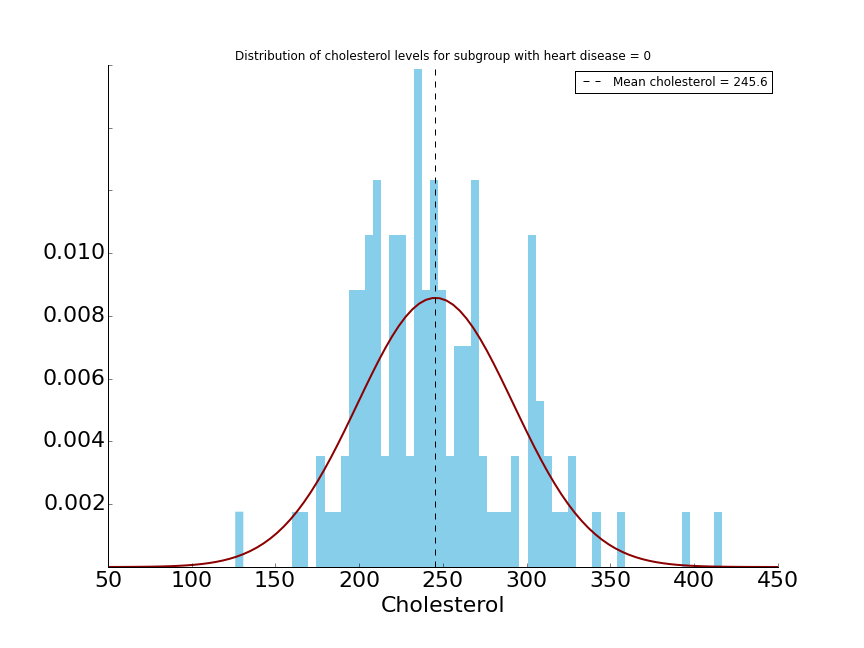
\includegraphics[scale = 0.5]{distribution_for_HD_0.png}

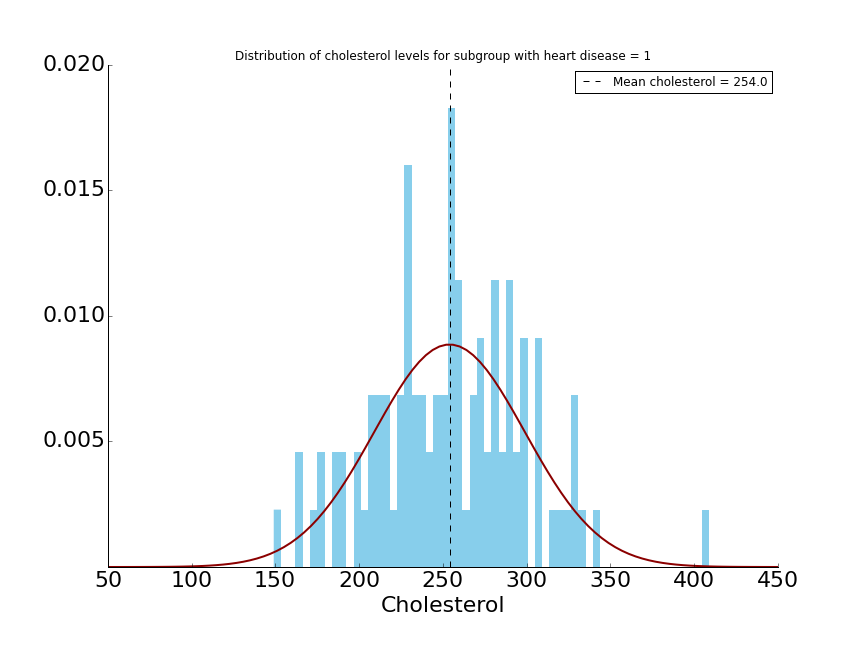
\includegraphics[scale = 0.5]{distribution_for_HD_1.png}

\subsection{Determining the error rate for our new MAP estimate}

Using our new MAP estimator trained on 218 observations, we misclassify 7 of the 50 patients in the test set. Thus, our error rate is 0.14. I trust this result, since it was determined using an out-of-sample test set.

\subsection{Questioning conditional independence assumptions}

We assumed the predictors were all conditionally independent given $H$. This assumption allowed us to estimate the probability distributions of predictors conditioned on only $H$. This is useful when the sample size is relatively small, because if the sample size is small and we don't make this assumption, then our conditional probability estimates for subgroups may become unstable. \\

To make this concrete, let's consider an example. In part (a), we used conditional independence to equate $P_{S|C, H}(s | c, h) = P_{S|H}(s | h)$. We then estimated this distribution by partitioning the 218 samples in the test set into four subsets ($R_S \times R_H$). If we had not made this assumption, we would have had to estimate the distribution of $P_{S|C, H}(s | c, h)$ by partitioning the 218 samples in the test set into 16 subsets ($R_S \times R_H \times R_C$). Given that each of these subsets would contain fewer numbers of samples, we would increase the variance in our model (due to greater variance in probability estimates). Moreover, this increase in variance would be even worse in part (d), where we added yet another feature to our model.\\

To conclude, we can relate this all back to a key concept in modeling, namely bias-variance tradeoff. By assuming conditional independence, we effectively decreased test variance (and avoided overfitting) at the expense of greater model bias (since, if the predictors are not conditionally independent, we have a misspecified model).
%----------------------------------------------------------------------------------------
\end{document}